
\chapter{Introduction}
\label{chapter:introduction}

Object orientation, while a boon to developer productivity, usually comes at the
expense of a degree of performance. When programming in this style, as we all do
when we code in Java, we make design choices that tend to favor small things.
We would rather write a large number of small methods than a small number of
large methods. Doing so usually results in methods that are individually easier
to understand. Having smaller methods is also nice, because they can be mixed
and matched, and thus reused more flexibly than monolithic code.

This style of coding methods actually isn't so bad for execution time, at least
not as bad as one would expect. As our code runs, a Just-in-Time (JIT) compiler
is busy optimizing away some of the overheads of having many small method
invocations. These optimizations, primarily method inlining, do a reasonable job
of reducing the penalty of coding in a object-oriented way. Performance may not
reach the ultimate levels of coding in a language such as C, but at least the
JIT has our back.

A similar situation occurs with memory consumption, though this story is not
nearly as rosy.
Modeling your data in Java is the process of designing how to map bytes of data
to fields and classes.
For example, an employee maps to a \class{Employee} Java class, and each
employee's identification number maps to an \class{int} field in that class. At
runtime, the Java Virtual Machine (JVM) will allocate an instance of that class,
thereby setting aside memory in the heap for its fields.

What happens if the identification number is not a scalar, but instead a mix of
numbers and characters? Even if the number is of fixed length, Java still forces
you to store this in an side array --- the language does not allow you to inline
that array into the \class{Employee} object itself. This means that, unless
your data is scalar primitives you pay the expense of allocating a new object,
and pointing to it. 

This cost, of \emph{delegation}, is around 16 bytes. You pay this cost for every
field of data that you choose, or are forced by the language, to delegate rather
than inline. The java runtime makes no attempt to inline that side array
for you. This lies in contrast to what the JIT does for methods: the JIT creates a
small number of larger methods by inlining small methods into larger ones.

This probably seems like height of madness, worrying about 16 bytes, in the age
of multi-gigabyte devices the size of your hand. It is true that a few bytes
here and there would not be worth the hassle, if these were costs paid only a
few times, or were small relative to the actual data you were trying to store.
Unfortunately, these overheads are not easily amortized, especially in a
language like Java.








\begin{comment}
After all, Java provides you with automatic garbage collection, and there are
lots of libraries and frameworks available, written by experts, that provide
powerful functionality. All you have to do is piece together the parts and let
the Java runtime system do the rest for you.

The reality, unfortunately, is very different. If you just assemble the parts, take
the defaults, and follow all the good advice to make your
program flexible and maintainable, you will likely find that your memory needs are
\emph{much} higher than imagined. You may also find that precious memory
resources are wasted holding on to data that is no longer needed, or, even
worse, that your system suffers from memory leaks. All too often, these problems
won't show up until late in the cycle, when the whole system comes together. 
You may discover, for example, when your product is about to ship, that your design is
far from fitting into memory, or that it does not support nearly the number
of users it needs to support. Fixing these problems can
take a major effort, requiring extensive refactoring or rethinking
architectural decisions, such as the choice of frameworks you use.
\end{comment}

\begin{comment}
[NOTE(GSS): In the next few paragraphs there's a lot of overlap with the
Preface.
Most of this material can be merged/moved into the preface. Let's 
get quickly to Facts and Fictions, which is very concrete.]

[NMM 20120625 i have moved this paragraph in part, to the preface]
This book is a guide to using memory wisely in Java. Memory usage,
like any other aspect of software, needs to be carefully
engineered. Predicting
your system's memory needs early in the cycle, and engineering with those needs in mind, can make
the difference between success and failure of your project. Engineering means making
informed tradeoffs, and, unfortunately, the information
to do so isn't always available. While there has been much written on how to
build systems that are bug-free, easy to maintain, and secure,
there is little guidance available on how to use Java memory efficiently
or even correctly. (Too often memory issues are left to chance, or at least
put off until there is a crisis.)  This book gives you the tools to make
informed choices early on.  It gives you 
an approach to looking at your system's uses of memory, and a practical guide
to making informed tradeoffs in every part of your design and
implementation. Java is also filled with
costly memory traps that are easy to fall into.  
 (Common patterns that make up your design - helps you understand costs and alternatives.  Also 
relevant Java mechanisms).  Three kinds of info: patterns, mechanisms, and an
organization/approach to thinking about memory.

(If you are like most Java developers, you probably don't have a good picture of
of how much memory your designs use.)
\end{comment}

% TODO put this somewhere later? NMM 20120625
\begin{comment}
Achieving efficient memory usage takes some effort in any language. 
There are things about Java that make it especially easy to end up with bloated
or even incorrect data designs. One reason is that Java is so easy to program,
so it gives you a false sense of security that everything is being handled for you. (Languages like C give you a
lot of control over storage, and so it is clear what
the consequences of your choices are.) Also, as we shall see,
the basic costs of building blocks such as Strings, can be surprisingly expensive,
when compared with languages like C++. So much is done for you in
Java, from management of the heap, to all the functionality hidden behind framework APIs, that it can be
difficult to find out how much memory your data structures need, or how long
they are staying around, until you have a fully running system. Compared to
many languages, Java also gives you fewer options for designing your data
structures and managing their storage. This means that if you find you have
problems, you have fewer ways of fixing them without rethinking larger aspects of your design.
All of this makes it important to understand what memory
costs and alternatives are, as early as possible.
\end{comment}

%\section{Facts and Fictions}
% [NOTE(GSS): Myths and Quiz go here.
% The underlying point (doesn't necessarily need to be stated) is why paying
% attention to costs etc. matters, and that it's possible to make a big
% difference.]

% [NOTE(GSS): Quiz can be a callout or scattered callouts.
% Doesn't have to be multiple choice. Maybe just a single answer, with an answer
% key on the next page.]

% Alternate Version 1:
%In addition to the technical reasons why managing memory can be a challenge,
% there are other reasons why memory footprint problems are so common. In particular,
%the software culture and popular beliefs can lead you to ignore memory
%costs. Some of these beliefs are really myths --- they might have once
%been true, but no longer. Here are several.
% Alternate Version 2:
% Beyond the technical realities of using memory well in Java there are some
% commonly held misconceptions that often make things worse. So before getting
% into how to engineer memory in Java, it is worth dispelling some of these
% myths, and getting a better understanding of why memory problems can be so
% common in Java.

A good example of this problem lies in the way Java represents the fundamental
data types, such as numbers and strings. The Java primitives are implemented in
Java. You may only have a thousand instances of your own data types, but your
heap is likely to contain millions of each of these primitives.

\callout{quiz1}{The Primitives that Aren't so Primitive}{
\noindent The Java standard
library ships with a suite of data types to handle the basic functionality of
representing numbers and strings. You might think that, being so elemental and
so widely used, that these would be highly optimized. Quite the opposite is
true.
\begin{itemize}
\item An \class{Integer} object consumes \emph{four} times more memory than its
non-object counterpart, the \class{int}, even if both represent the same piece
of data: 16 bytes versus 4 bytes.
\item A \class{String} object that represents 8 characters consumes \emph{four}
times more memory than the characters themselves, and \emph{eight} times more memory
than if these were represented as ASCII characters.
\item A \class{Date} object consumes FIXME times more memory than the 4 bytes
worth of information it represents.
\end{itemize}
}



%The overhead of these primitive data types is high. Doing better is possible,
%but, within the constraints of the Java language, and following principled
%object orientation, doing so takes some forethought.

Another basic building block of Java programs is the collections. The use
collections is unavoidable, but, with some planning, you can avoid wasting space
on the overhead of the collection implementations.

\callout{quiz2}{Surprisingly Expensive Collections}{ The standard Java
collections library offers implementations of sets, maps, and lists. These are
all implemented in Java, and often come at a high expense.
The expense comes in two forms: the overhead of for each entry, and the overhead
for each collection.

\begin{itemize}
  \item Each \class{HashSet} costs 104 bytes, plus 24 bytes of overhead for
  each entry. This is more expensive than the more functional \class{HashMap}.
  %, which  costs 88 bytes per collection.
  \item If you have a large number of small sets, the per-collection cost
  dominates. By restructuring to have a small number of large sets, or
  by choosing a more efficient representation of small sets, you can reduce
  overhead by a factor of 5.
  %\item If your heap contains 100 sets with an average of 10000 entries, you
  % will waste 244 kilobytes on collection overhead.
  %\item If your heap contains the same total number of entries, but with an
  % average of only 10 entries per collection, you will waste 10 megabytes on
  % overhead --- this is an order of magnitude worse.
\end{itemize}
}



The overheads of primitives and collections each are bad on their own. The
problem of overhead multiplies when you combine them. This is a frequent
occurrence, given the way we all program these days. Applications are an
assemblage of reuseable code. The standard \class{HashSet} is a subclass of
\class{HashMap}, well, because, logically, that is an essential truth: a set is
a map with a null value. We make these choices, in favor of reuse rather than
specialization, at every juncture. As the process of assembling code proceeds,
these choices being to pile up, usually at the expense of memory consumption.

\callout{quiz3}{The Big Pileup}{
Primitive data types are expensive, as is storing data in the standard
collections comes with a high overhead. The story gets worse as you combine them
into larger data structures. With each added layer, expenses pile up. Let's say
that you want to store one million pieces of information. 
\begin{itemize}
  \item In a language like \CC, short strings, say 8 ASCII characters a piece,
  stored in a simple array will consume \textbf{11} megabytes. %((4 + 8)*1000000 + 12)/1024/1024
  \item In Java, this example consumes \textbf{61} megabytes, % ((4 +
  % 28+16+8*2)*1000000 + 12)/1024/1024
  a factor of 5.5x more expensive.
  \item These same strings stored in a \class{HashSet} consume \textbf{80}
  megabytes, %((24 + 28+16+10*2)*1000000 + 104)/1024/1024
  an extra factor of 31\%.
  \item If the elements are instead a class wrapped around a single string, this 
  consumes \textbf{95} megabytes. %((24 + 16 + 28+16+10*2*4)*1000000 +% 104)/1024/1024
  You pay an extra 18\% for the luxury of that wrapper object. 
  \item If the elements are each a set with on average a single string, this
  consumes \textbf{202} megabytes. %((24 + 104 + 24 + 28+16+10*2*4)*1000000 + 104)/1024/1024
\end{itemize}
}

\begin{wrapfigure}{r}{0.5\textwidth}
	\vspace{-2.25em}
	\centering
	\subfigure[C++]{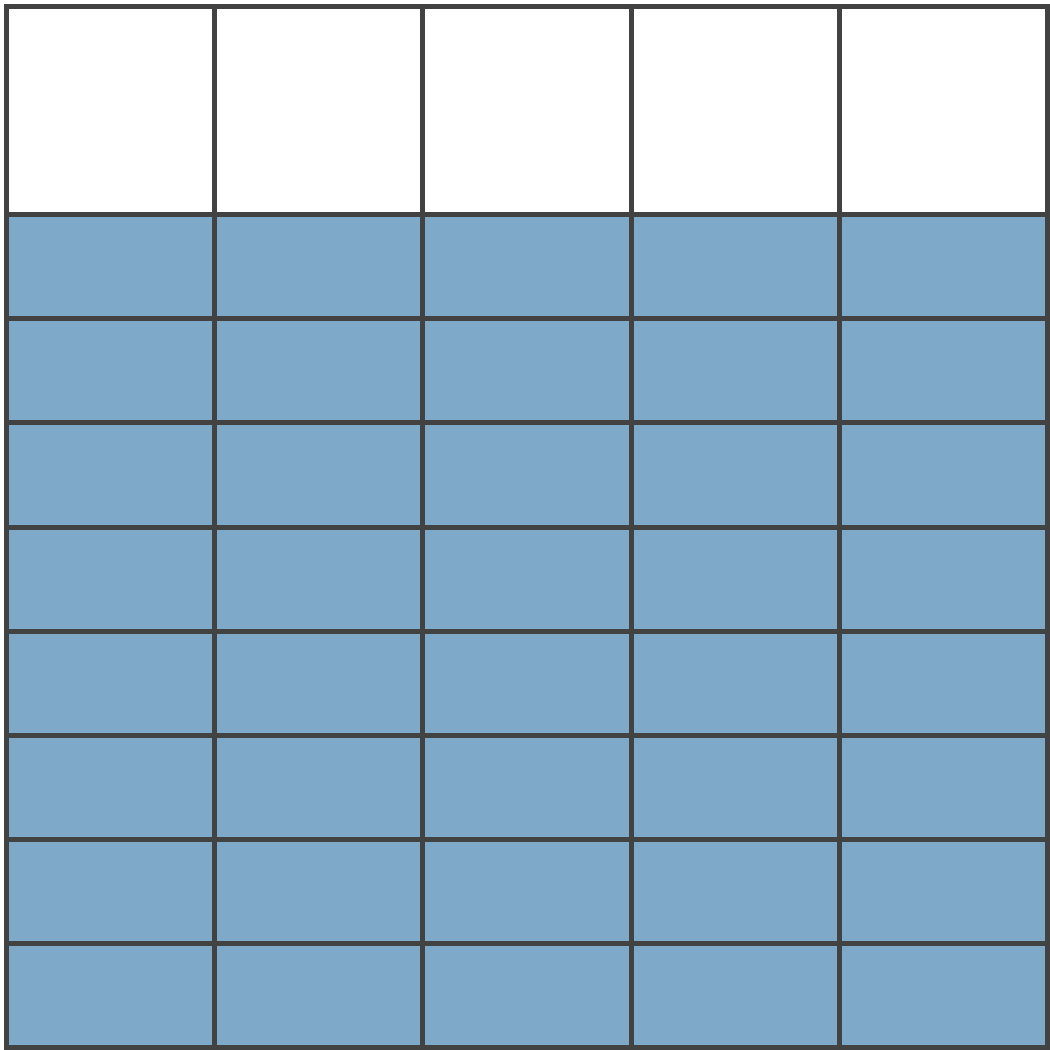
\includegraphics[width=0.2\textwidth]{Figures/c++_density}}
	\qquad
	\subfigure[Java]{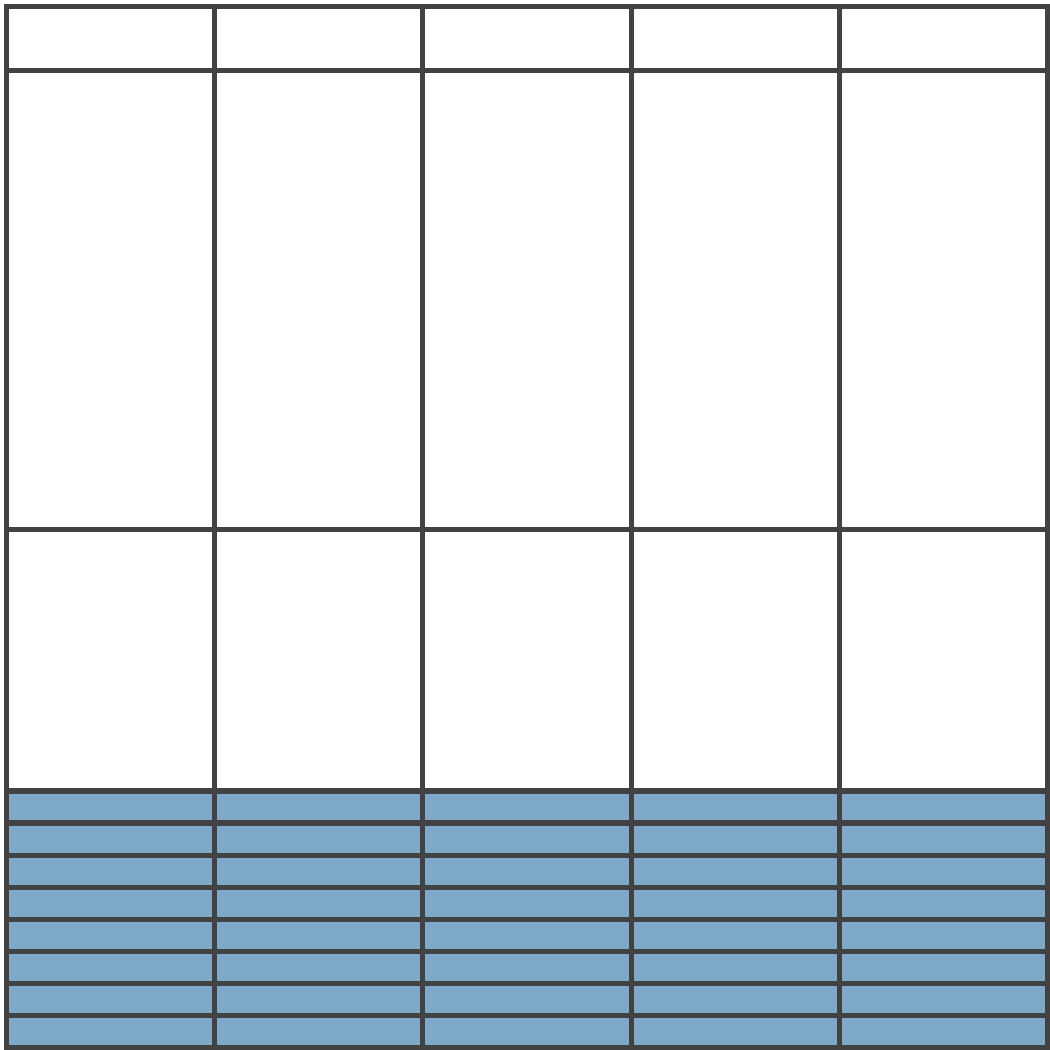
\includegraphics[width=0.2\textwidth]{Figures/java_density}}
	\caption{The density of actual data (shown in the darker shade) versus
	the overhead of storing data when storing 8-character strings
	in an array: C++ versus Java.
	}
	\label{fig:c++_versus_java_density}
\end{wrapfigure}

Who would be so silly as to choose anything but the first way of storing these
strings? Welcome to the wonderful world of Java! In various forms, we have seen
all of these in real, deployed applications. However, you needn't resign
yourself to high memory consumption, because, with a bit of design work, there
is usually huge room for improvement. Keeping an eye on the \emph{density} of
actual data, relative to the overheads of storing that data, is a key to healthy
design. \autoref{fig:c++_versus_java_density} illustrates the first two of these
examples, elided to show just the first five entries of the array. 

High memory consumption is problematic when it forces expenditures for extra RAM
and machines, but grows even more troublesome when it leads to application
failures due to heap exhaustion. Sometimes, this is due to a design that
requires the entire data set to be in memory at one time, but a lack of
available Java heap to contain it all. Other times, your application runs out of
memory because of a memory leak.

\callout{quiz4}{Memory Leaks in a Managed Runtime}{ Java is often referred to as
having a \emph{managed runtime}. An important part of this is automatic garbage
collection. The standard sales pitch here claims that manual reclamation of
memory isn't required, and, for the most part, this is actually true.
\begin{itemize}
  \item With a publish/subscribe mechanism, you need to carefully
  manage the subscription list. If subscribers forget to deregister, then you
  will leak all objects that are transitively pointed to by the object that
  represents that subscriber.
  \item In caches with a sizing policy that is a function of the
  number of entries, rather than the total memory consumed by the entries, there
  is a good chance that the memory consumed by the cache will, at some point,
  exceed available heap capacity.
  \item Race conditions can also result in code that is no longer accessible by
  the program, but is \emph{reachable}, i.e. considered alive by the garbage
  collector. These orphaned objects will stay around for the duration of the
  run, and possibly accumulate over time.
%  If
  %you implement a nested set of maps, such as to handle a multi-part key, and a
  % race condition results in one thread overwriting the nested map for the
  % primary key, then the secondary map will no longer be accessible,
  %even though it is \emph{reachable}.
\end{itemize}
}

% [NMM 20120627] i think it might be good to have this section title be the same
% as the title of the book, or nearly so
\section{\thetitle}

%[NOTE(GSS): this is our approach, with a roadmap of the book.
%Needs to be rewritten/restructured to reflect our current breakdown: space,
%lifetime, scalability.]

%[NOTE(GSS): Somewhere in here will be a description of bloat factor and of E-C
%diagrams.  Just a high-level description of each in the Intro, detailed
%descriptions and examples are in Chapter 2.]

Central to good design is a keen focus on understanding your requirements.
In the context of memory consumption, there are important aspects of your needs
to keep in mind. Do you need random access into this data? Will entries ever be
deleted from collections? Does this entry need to remain alive for the duration
of the program? Which collections will grow larger as various aspects of load
increase? The book will guide you through these design requirement questions,
with a constant focus on common patterns that come up in practice. It shows you
how to recognize these patterns in your designs, and give you relevant
information about costs and other pitfalls.

Throughout the course of this book, you will learn three skills, to aid you in
designing more efficient data models:
\begin{enumerate}
  \item Estimating memory efficiency with simple back-of-the-envelope
  calculations.
  \item Recognizing common patterns of memory usage.
  \item Using the mechanisms that Java provides in order to properly manage the
  lifetime of your objects, thus avoiding memory leaks, and manage data models
  that do not fit into the Java heap.
\end{enumerate} 

% probably overkill:
%\dividingline

%\subsection{Estimating the Efficiency of Your Design}
%discuss estimating (Edith text on counting bytes, etc is great) (including
%   scalability discussion) (and focusing on important stuff)
%discuss health very briefly
%discuss entities and collections

\autoref{part:1} presents the issues of estimating memory efficiency.
\autoref{chapter:memory-health} shows you how to compute an accounting metric,
the \textbf{Bloat Factor}, which measures the density of actual data in your
data models. Memory spent on pointers, and on headers that the Java runtime
tacks on to every object, are not absolutely necessary parts of a design. Poor
designs will waste more space on these overheads, and thus have a high bloat
factor. If you read only one chapter of this book,
\autoref{chapter:memory-health} is the one to focus on.

\autoref{chapter:memory-health} also introduces a diagramming technique, the
\textbf{Entity-Collection Diagram}, that aids in determining these costs, and in
comparing the amount of bloat in design alternatives.
An E-C Diagram makes explicit the two key aspects of the health of a design:
% highlights the major elements of the data model implementation, so that the
% costs and scaling consequences of the design are easily visible.
% These diagrams appear throughout the book to illustrate various implementation
% options and their costs.
the implementations of the \emph{entities} of your application, such as your
business objects, and way you have chosen to associate them using collections.
% The kinds of choices you make to improve the storage of your entities are
% often different from those Collections are also depicted as nodes, using an
% octagonal shape.
This is different from UML class diagrams, where associations are shown as
edges.
\autoref{chapter:delegation} through
% \autoref{chapter:field-patterns},\autoref{chapter:representing-values},
\autoref{chapter:sharing-immutable-data} cover issues related to the design of
entities.
\autoref{chapter:brief-introduction-collections} through
% \autoref{chapter:representing-relationships},
% \autoref{chapter:tables-indexes},
\autoref{chapter:dynamic-records} help with planning out to use off-the-shelf
collections, and also with the design of new collections libraries.

% discuss looking at each data structures separately [NMM ??]

\begin{comment}
[NMM 20120628 too much E-C diagram detail for intro?]
A data model implementation begins with a conceptual understanding of the
entities and relationships in the model.  This may be an informal understanding,
or it may be formalized in a diagram such as an E-R diagram or a UML class
diagram.  At some point that conceptual model is turned into Java classes that
represent the entities, attributes, and assocations of the model, as well as any
auxiliary structures, such as indexes, needed to access the data.  The example
below shows a simple conceptual model, using a UML class diagram.  A Java
implementation of that model is also shown, using rectangles for classes and
arrows for references.  %The Java diagram below is typical of a schema diagram,
in that it shows
\end{comment}

% probably overkill:
%\dividingline

\autoref{part:2} discusses managing the lifetime of objects. In
\autoref{chapter:lifetime-requirements}, you will learn how to establish the
lifetime requirements of your data, by mapping your needs to one of four common
lifetime patterns: temporaries, permanently resident objects, objects with
correlated lifetimes, and objects that represent a time-space trade-off.
\autoref{chapter:lifetime-fundamentals} provides a primer on the memory
management facilities that Java offers.
\autoref{chapter:lifetime-implementation-strategies} and
\autoref{chapter:trading-space-for-time} focus on the last two of these lifetime
patterns.

% probably overkill:
%\dividingline

In addition to determining the bloat factor of individual data structures and
avoiding memory leaks, it is important to estimate how well the overall design
will scale up as load increases. The final part of this book, \autoref{part:3},
covers issues related to the scalability of your designs.
\autoref{chapter:estimating-scalability} teaches you strategies for estimating
the scalability of a design, given an E-C Diagram.
\autoref{chapter:large-long-lived} covers the cases when your data model still
does not fit, even after applying the tuning methodology of \autoref{part:1}.
Sometimes you need to tear down the elements of the facade of object
orientation, and this is entirely possible while remaining largely within the
confines of Java, and without resorting to the use of secondary storage.
Finally, \autoref{chapter:secondary-stores} gives strategies for the case when
you must resort to the use of disk or remote storage in order to make your data
fit.




\begin{comment}
\section{Conventions Used in This Book}

[NOTE(GSS): add data structure to the list.  possibly add relationship as well.]

Terms like object can have different meanings in the literature.  The following are the conventions used throughout this book.

\begin{itemize}
\item A \textit{class} is a Java class. A class name, for example \texttt{String}, always appears in type-writer font. 
\item A \textit{data model} is a set of classes that represents one or more logical concepts.
\item Finally, an \textit{object} is an instance of a class, that exists at runtime occupying a contiguous section of memory.
\end{itemize} 
\end{comment}





\begin{comment}
 % NICK's NOTES
microscopic estimating (field-level counting), and accounting to predict
scale

EC diagram, bloat factory, scaling, 

lifetime: sometimes it's not a leak, just a consumption problem (in-memory
design, didn't fit)

sometimes optimizations cost: making a side object for rarely used fields; when
is it useful sharing immutable data (how much sharing before factoring it out
is worthwhile)

what java gives you, what it doesn't, some things are kinda hard to use; java
makes it hard for you

you actually have control



preface

things are hard to change at some point. it's easy to get to an irreconciliable
spot.

intro

why isn't this just for systems programmers making b-trees? this is about
everyday application development

i have GC, why care about lifetime?
i have standard data structures, why care about data model design?

data modeL: entites and relations

visual presentation of density
[flyweight: canonicalizing map]
\end{comment}